\begin{figure}[H]
\centering
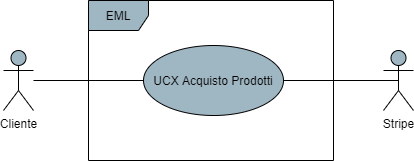
\includegraphics[scale=0.6]{res/UseCase/Immagini/AcquistoProdottiGenerale}
\caption{Diagramma UML\ped{G} per modulo di acquisto prodotti}
\end{figure}

\subsubsection{UC7 - Acquisto prodotti}
\begin{itemize}
\item \textbf{Attori primari}: cliente;
\item \textbf{Attori secondari}: Stripe\ped{G};
\item \textbf{Descrizione}: il cliente può acquistare i prodotti presenti nel suo carrello;
\item \textbf{Scenario Principale}: 
\begin{enumerate}
	\item il cliente inizia il checkout dei prodotti nel carrello \textbf{[UC7.1]};
	\item il cliente verifica l'indirizzo email e inserisce i dati per il pagamento \textbf{[UC7.3]};
	\item il cliente procede al pagamento \textbf{[UC7.4]};
	\item il cliente visualizza un riepilogo dell'ordine effettuato \textbf{[UC7.7]};
\end{enumerate}
\item \textbf{Precondizione}: l'utente è autenticato come cliente, si trova nella pagina del carrello e ha precedentemente inserito dei prodotti nel carrello;
\item \textbf{Postcondizione}: il costo totale dei prodotti acquistati è stato prelevato dal conto specificato dal cliente. È stata inviata un'email al cliente per confermare l'acquisto.
\end{itemize}

\begin{figure}[H]
\centering
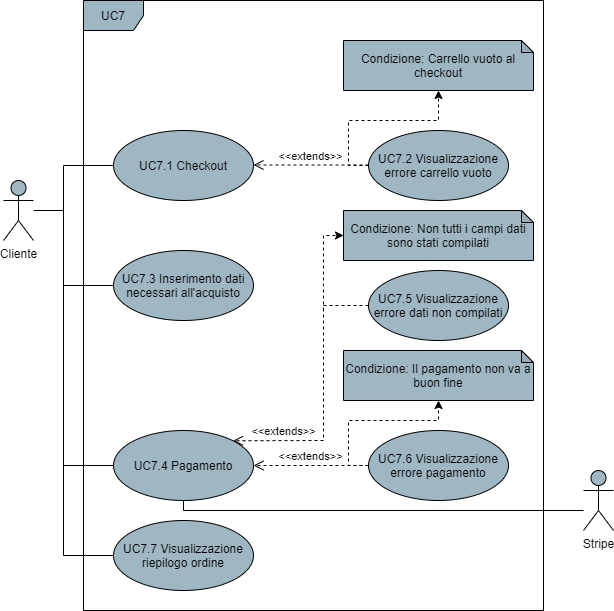
\includegraphics[scale=0.6]{res/UseCase/Immagini/AcquistoProdotti}
\caption{Diagramma UML\ped{G} per UC7 - Acquisto prodotti}
\end{figure}

\subsubsection{UC7.1 - Checkout}
\begin{itemize}
\item \textbf{Attori primari}: cliente;
\item \textbf{Descrizione}: il cliente effettua il checkout per iniziare la procedura di acquisto prodotti;
\item \textbf{Scenario Principale}: il cliente preme il bottone dedicato al checkout, nella pagina del carrello;
\item \textbf{Estensioni}:
\begin{itemize}
\item se non è presente alcun prodotto nel carrello viene visualizzato un messaggio di errore \textbf{[UC7.2]};
\end{itemize}
\item \textbf{Precondizione}: l'utente è autenticato come cliente, si trova nella pagina del carrello e ha premuto il bottone dedicato al checkout;
\item \textbf{Postcondizione}: il cliente viene reindirizzato alla pagina di verifica email e di pagamento, dove può continuare l'acquisto dei prodotti.
\end{itemize}

\subsubsection{UC7.2 - Visualizzazione errore carrello vuoto}
\begin{itemize}
\item \textbf{Attori primari}: cliente;
\item \textbf{Descrizione}: il cliente visualizza un messaggio di errore che lo informa che per procedere al checkout è necessario avere almeno un prodotto nel carrello;
\item \textbf{Scenario Principale}: il cliente prova ad effettuare il checkout senza aver precedentemente inserito prodotti nel suo carrello;
\item \textbf{Precondizione}: il cliente si trova nella pagina del carrello e ha premuto il bottone dedicato al checkout;
\item \textbf{Postcondizione}: viene visualizzato un messaggio che informa il cliente della necessità di avere almeno un prodotto nel carrello per iniziare il checkout.
\end{itemize}

\subsubsection{UC7.3 - Inserimento dati necessari all'acquisto}
\begin{itemize}
\item \textbf{Attori primari}: cliente;
\item \textbf{Descrizione}: il cliente compila i campi dati necessari all'acquisto dei prodotti selezionati;
\item \textbf{Scenario Principale}: il cliente si trova nella pagina di pagamento e, per concludere l'acquisto, inserisce i seguenti dati:
\begin{itemize}
	\item il cliente verifica l'indirizzo email indicato in fase di registrazione \textbf{[UC7.3.1]} o può indicarne uno diverso per l'invio dell'email di conferma acquisto \textbf{[UC7.3.2]};
	\item il cliente inserisce i dati relativi al metodo di pagamento, come nome, cognome e numero di carta di credito \textbf{[UC7.3.3]};
\end{itemize}
\item \textbf{Precondizione}: il cliente ha superato il checkout e si trova nella pagina di pagamento;
\item \textbf{Postcondizione}: il cliente può continuare il pagamento e l'acquisto.
\end{itemize}

\begin{figure}[H]
\centering
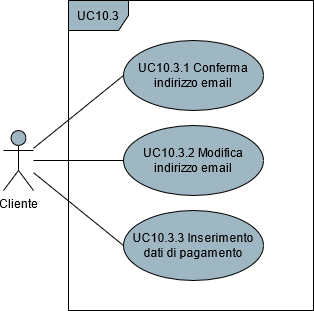
\includegraphics[scale=0.6]{res/UseCase/Immagini/InserimentoDatiAcquisto}
\caption{Diagramma UML\ped{G} per UC7.3 - Inserimento dati necessari all'acquisto}
\end{figure}

\subsubsection{UC7.3.1 - Verifica indirizzo email di spedizione}
\begin{itemize}
\item \textbf{Attori primari}: cliente;
\item \textbf{Descrizione}: il cliente verifica l'indirizzo email inserito durante la fase di registrazione;
\item \textbf{Scenario Principale}: il cliente visualizza l'indirizzo email precedentemente inserito, che verrà utilizzato per l'invio dell'email di conferma acquisto;
\item \textbf{Precondizione}: il cliente ha superato il checkout e si trova nella pagina di pagamento;
\item \textbf{Postcondizione}: il cliente visualizza e verifica il suo indirizzo email.
\end{itemize}

\subsubsection{UC7.3.2 - Modifica indirizzo email di spedizione}
\begin{itemize}
\item \textbf{Attori primari}: cliente;
\item \textbf{Descrizione}: il cliente modifica l'indirizzo email inserito durante la fase di registrazione;
\item \textbf{Scenario Principale}: il cliente può modificare l'email per la conferma dell'acquisto, sovrascrivendo l'indirizzo visualizzato \textbf{[UC7.3.1]};
\item \textbf{Precondizione}: il cliente ha superato il checkout, si trova nella pagina di pagamento e visualizza il campo dati dedicato alla verifica dell'indirizzo email \textbf{[UC7.3.1]};
\item \textbf{Postcondizione}: il cliente modifica il suo indirizzo email, sovrascrivendo quello visualizzato.
\end{itemize}

\begin{figure}[H]
\centering
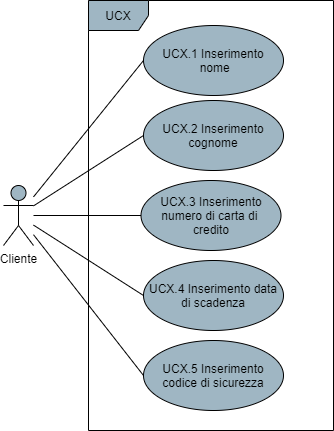
\includegraphics[scale=0.6]{res/UseCase/Immagini/InserimentoDatiPagamento}
\caption{Diagramma UML\ped{G} per UC7.3.3 - Inserimento dati di pagamento}
\end{figure}

\subsubsection{UC7.3.3 - Inserimento dati di pagamento}
\begin{itemize}
\item \textbf{Attori primari}: cliente;
\item \textbf{Descrizione}: il cliente inserisce i dati relativi alla sua carta di pagamento;
\item \textbf{Scenario Principale}: il cliente inserisce nel form relativo ai dati di pagamento le seguenti informazioni:
\begin{itemize}
	\item nome collegato al conto \textbf{[UC7.3.3.1]};
	\item cognome collegato al conto \textbf{[UC7.3.3.2]};
	\item numero di carta \textbf{[UC7.3.3.3]};
	\item mese e anno di scadenza della carta \textbf{[UC7.3.3.4]};
	\item codice di sicurezza \textbf{[UC7.3.3.5]};
\end{itemize}
\item \textbf{Precondizione}: il cliente ha superato il checkout e si trova nella pagina di pagamento;
\item \textbf{Postcondizione}: il cliente ha compilato i dati di pagamento.
\end{itemize}

\subsubsection{UC7.3.3.1 - Inserimento nome}
\begin{itemize}
\item \textbf{Attori primari}: cliente;
\item \textbf{Descrizione}: il cliente inserisce nelle informazioni richieste per il pagamento il nome;
\item \textbf{Scenario Principale}: il cliente inserisce nel form relativo ai dati di pagamento il nome collegato al conto;
\item \textbf{Precondizione}: il cliente ha superato il checkout e si trova nella pagina di pagamento;
\item \textbf{Postcondizione}: il cliente ha compilato il campo dati dedicato al nome.
\end{itemize}

\subsubsection{UC7.3.3.2 - Inserimento cognome}
\begin{itemize}
\item \textbf{Attori primari}: cliente;
\item \textbf{Descrizione}: il cliente inserisce nelle informazioni richieste per il pagamento il cognome;
\item \textbf{Scenario Principale}: il cliente inserisce nel form relativo ai dati di pagamento il cognome collegato al conto;
\item \textbf{Precondizione}: il cliente ha superato il checkout e si trova nella pagina di pagamento;
\item \textbf{Postcondizione}: il cliente ha compilato il campo dati dedicato al cognome.
\end{itemize}

\subsubsection{UC7.3.3.3 - Inserimento numero di carta di credito}
\begin{itemize}
\item \textbf{Attori primari}: cliente;
\item \textbf{Descrizione}: il cliente inserisce nelle informazioni richieste per il pagamento il numero di carta;
\item \textbf{Scenario Principale}: il cliente inserisce nel form relativo ai dati di pagamento il numero di carta di credito;
\item \textbf{Precondizione}: il cliente ha superato il checkout e si trova nella pagina di pagamento;
\item \textbf{Postcondizione}: il cliente ha compilato il campo dati dedicato al numero di carta di pagamento.
\end{itemize}

\subsubsection{UC7.3.3.4 - Inserimento data di scadenza}
\begin{itemize}
\item \textbf{Attori primari}: cliente;
\item \textbf{Descrizione}: il cliente inserisce nelle informazioni richieste per il pagamento il mese e l'anno di scadenza della carta di credito;
\item \textbf{Scenario Principale}: il cliente inserisce nel form relativo ai dati di pagamento mese e l'anno di scadenza della carta;
\item \textbf{Precondizione}: il cliente ha superato il checkout e si trova nella pagina di pagamento;
\item \textbf{Postcondizione}: il cliente ha compilato il campo dati dedicato alla data di scadenza.
\end{itemize}

\subsubsection{UC7.3.3.5 - Inserimento codice di sicurezza}
\begin{itemize}
\item \textbf{Attori primari}: cliente;
\item \textbf{Descrizione}: il cliente inserisce nelle informazioni richieste per il pagamento il codice di sicurezza;
\item \textbf{Scenario Principale}: il cliente inserisce nel form relativo ai dati di pagamento il codice di sicurezza collegato alla carta di credito;
\item \textbf{Precondizione}: il cliente ha superato il checkout e si trova nella pagina di pagamento;
\item \textbf{Postcondizione}: il cliente ha compilato il campo dati dedicato al codice di sicurezza.
\end{itemize}

\subsubsection{UC7.4 - Pagamento}
\begin{itemize}
\item \textbf{Attori primari}: cliente;
\item \textbf{Attori secondari}: Stripe\ped{G};
\item \textbf{Descrizione}: il cliente procede all'ordine. Il pagamento viene effettuato tramite Stripe\ped{G}, che riporterà l'esito ed eventuali errori;
\item \textbf{Scenario Principale}: il cliente conferma l'ordine tramite l'apposito bottone;
\item \textbf{Estensioni}:
\begin{itemize}
	\item l'utente non ha compilato tutti i campi necessari al pagamento. Il cliente visualizza un messaggio di errore che lo informa della necessità di inserire tutti i dati per procedere al pagamento \textbf{[UC7.5]};
	\item il pagamento non va a buon fine. Il cliente visualizza un messaggio di errore contenente le cause del fallimento \textbf{[UC7.6]}.
\end{itemize}
\item \textbf{Precondizione}: il cliente si trova nella pagina di pagamento;
\item \textbf{Postcondizione}: il costo totale dei prodotti acquistati è stato prelevato dal conto specificato dal cliente. È stata inviata un'email al cliente per confermare l'acquisto. Al cliente viene mostrato un riepilogo dell'ordine appena effettuato.
\end{itemize}

\subsubsection{UC7.5 - Visualizzazione errore dati non compilati}
\begin{itemize}
\item \textbf{Attori primari}: cliente;
\item \textbf{Descrizione}: il cliente visualizza un messaggio di errore che lo informa della necessità di compilare tutti i campi dati per procedere al pagamento;
\item \textbf{Scenario Principale}: il cliente preme il bottone dedicato al pagamento senza prima aver compilato tutti i campi richiesti;
\item \textbf{Precondizione}: il cliente si trova nella pagina di pagamento e non ha compilato tutti i campi dati necessari per procedere all'acquisto;
\item \textbf{Postcondizione}: viene visualizzato un messaggio che informa il cliente dell'errore e che consiglia all'utente di controllare i dati inseriti e riprovare.
\end{itemize}

\subsubsection{UC7.6 - Visualizzazione errore pagamento}
\begin{itemize}
\item \textbf{Attori primari}: cliente;
\item \textbf{Attori secondari}: Stripe\ped{G};
\item \textbf{Descrizione}: il cliente visualizza un messaggio di errore che lo informa del motivo per il fallimento del pagamento. L'utente può poi controllare i dati inseriti e ritentare il pagamento;
\item \textbf{Scenario Principale}: il cliente prova ad effettuare il pagamento inserendo dati di una carta che per qualche motivo rifiuta l'addebito;
\item \textbf{Precondizione}: il cliente si trova nella pagina di pagamento e ha compilato i campi dati necessari per procedere all'acquisto;
\item \textbf{Postcondizione}: viene visualizzato un messaggio che informa il cliente dell'errore avvenuto nel processo di pagamento, consigliandogli di controllare i dati inseriti e riprovare.
\end{itemize}


\subsubsection{UC7.7 - Visualizzazione riepilogo ordine}
\begin{itemize}
\item \textbf{Attori primari}: cliente;
\item \textbf{Descrizione}: il cliente visualizza un riepilogo dell'ordine appena effettuato contenente l'elenco di prodotti, ognuno con prezzo e quantità, il costo totale, le tasse, l'indirizzo di spedizione e la data;
\item \textbf{Scenario Principale}: il cliente ha effettuato un ordine e ne visualizza un riepilogo;
\item \textbf{Precondizione}: il cliente ha completato un ordine ed il pagamento è andato a buon fine;
\item \textbf{Postcondizione}: viene visualizzato un riepilogo dell'ordine effettuato.
\end{itemize}
